\chapter{Preliminary concepts}

\section{Dynamical Systems}

[introducir bien el tema]. 

The general form for a dynamical system is the following.

\begin{equation}
    \dfrac{d\bm{u}}{dt} = \bm{f}(\bm{u}, \eta), \qquad \bm{f} : \mathbb{R}^N \times \mathbb{R}^{n_\eta} \to \mathbb{R}^N
    \label{eq:def_ds}
\end{equation}

Here, $\bm{u}$ represents the state vector of the system, it might correspond to the
concentrations of different chemicals, the population of certain species or the amplitude
of an electric field. The temporal evolution of the state of the system is thus determined by 
the vector function $\bm{f}$. This function may, in turn, depend on one or more control
parameters $\eta$ relevant to the modeled experiment (i.e. driving frequency, pumping power, etc).

In this thesis, different dynamical systems in the form of Eq.~(\ref{eq:def_ds}) with a {\em nonlinear} function
$\bm{f}$ will be considered. Although it might be argued that, at a fundamental level, the physical laws
that describe the evolution of a system are linear (such as the Schrödinger equation), when one looks at meso- or macroscopical
systems, nonlinear terms naturally arise due to the coarse-graining of the microscopical degrees of freedom [ref Karadr].


In the case of a nonlinear dynamical system, it becomes extremely difficult, and often impossible, to find
general explicit solutions of Eq.~(\ref{eq:def_ds}). But it turns out that in most cases, an in-depth
description of the model can be provided by studying only the steady states ($\bm{f}(\bm{u}, \eta) = 0$) and their qualitative changes as parameters 
are varied. In other words, the problem can be reduced to finding the {\em equilibria} and {\em bifurcations} of the system.
In the following section, the elementary bifurcations a system can experience will be described.

\section{Bifurcations}

Qualitative changes of equilibria as parameters are varied.

% Ideas:
% \begin{enumerate}
%     \item saddle-node for genes pp 249
%     \item magnetism Landau Pitchfork
%     \item Hopf, van der pol, bici
% \end{enumerate}

\subsection{Saddle-Node bifurcation}

{\em Saddle-node} or {\em fold} bifurcations provide the simplest mechanism 
for which a pair of stable and unstable equilibria can be created (or destroyed) 
as the control parameter is changed. Although they arise in a huge variety of systems 
[insert ref], close to the bifurcation point the dynamics can always be reduced to
the following minimal or {\em normal form}.

\begin{equation}
    \dfrac{du}{dt} = \eta - u^2
    \label{eq:pre_bif_sn}
\end{equation}

Following the notation of Eq.~(\ref{eq:def_ds}), u represents the state variable
and $\eta$ the control parameter. For $\eta > 0$, the system presents two equilibria $u_{\pm} = \pm\sqrt{\eta}$, where $u_+$ is
stable and $u_-$ unstable. An interesting case occurs when $\eta = 0$, at which point $u = 0$ is
half-stable (stable for positive perturbations and unstable for negative perturbations). Lastly,
for $\eta < 0$ there are no equilibria. Figure~(\ref{fig:pre_bifs_sn}) provides a visual representation
of the previous analysis.

In short, as the bifurcation parameter $\eta$ is decreased (increased)
starting from positive (negative) values, the two equilibria attract (repel) each other and suddenly annihilate (appear).

\begin{figure}[h]
    \centering
    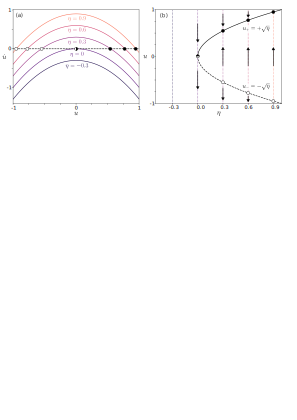
\includegraphics[width=\textwidth]{imagenes/framework/bif_sn_f.pdf}
    \caption{Prototipical scenario for a saddle-node bifurcation. (a) Phase space
    showing both stable and unstable fixed points for different values of $\eta$. 
    Black (white) circles represent
    stable (unstable) fixed points. (b) Bifurcation diagram showing
    the creation of a stable-unstable pair of fixed points. Solid (dashed) line represents
    stable (unstable) branch.}
    \label{fig:pre_bifs_sn}
\end{figure}

\begin{exmp}
    For centuries, the mystery of synchronization between fireflies has
    captivated many people. Although many open questions remain on this topic [ref],
    we will aim to shed {\em light} on this topic only with the knowledge of saddle-node bifurcations
    and a simple model proposed by Ermentrout and ...[ref]. 
    
    Consider the problem
    of a firefly flashing under the presence of a periodically flashing light.
    We will model the flashing of the firefly with an angular variable $\theta$
    such that $\theta = 0$ represents the firefly's flash. The firefly has its 
    own inherent frequency $\omega$, i.e. in the absence of stimuli 
    $\dot{\theta} = \omega$. On the other hand, the periodic stimulus will be
    represented by a phase $\phi$ that satisfies $\dot{\phi} = \Omega$, where 
    $\Omega$ is of course the stimuli period. In order to synchronize with the
    stimuli, the firefly will either want to speed up if it is lagging behind
    or slow down if it is going too fast. The simplest non-linear model that
    fulfills these assumptions is the following,
    \begin{align*}
        \dot{\phi} &= \Omega \\
        \dot{\theta} &= \omega + A \sin(\phi -  \theta)
    \end{align*}

    Subtracting both equations and defining $\varphi = \dot{\phi} - \dot{\theta}$
    yields 

    \begin{equation*}
        \dot{\varphi} = \Omega - \omega - A \sin \varphi
    \end{equation*}

    which can be adimensionalized by rescaling $t \to At$ and introducing
    the non-dimensional parameter $\mu = (\Omega - \omega)/A$,

    \begin{equation}
        \dot{\varphi} = \mu - \sin \varphi
        \label{eq:pre_bif_sn_exmp}
    \end{equation}

    For $\mu = 0$ where the forcing and intrinsic frequencies are the same, there
    is a stable fixed point at $\varphi = 0$ and an unstable fixed point at $\varphi = \pi$.
    As $\mu$ increases, both equilibria approach each other until they collide for $\mu=\mu_c=1$
    at $\varphi = \pi/2$
    and then disappear for $\mu > 1$. We can recognize that the pair of fixed
    points appear (or disappear) through a saddle-node bifurcation.
    
    Moreover, close to the bifurcation point where $\mu_c = 1$ and $\varphi_c = \pi/2$,
    we can do a Taylor expansion: $\mu = 1 + \eta$ and $\varphi = \pi/2 + u$ 
    where $\eta, u \ll 1$. Using the identity $\sin \varphi = \sin (\pi/2 + u) = \cos u$
    and inserting the previous ansatz into Eq.~(\ref{eq:pre_bif_sn_exmp}) yields
    the following
    \begin{align*}
        \dot{\varphi} = \dot{u} &= 1 + \eta - \cos u \\ 
        &\approx 1 + \eta - (1 - \dfrac12 u^2) \\
        &= \eta - \dfrac12 u^2
    \end{align*}

    Which after adequate rescaling corresponds exactly with the saddle-node
    normal form.
    

\end{exmp}

\subsection{Pitchfork bifurcation}

{\em Pitchfork} bifurcations typically arise in systems with symmetry and 
provide a universal mechanism for symmetry-breaking [ref strogatz]. 
A simple example is given by the statistical description of magnetization. 
In the absence of an external field, the net magnetization $m$ 
(below the critical temperature $T_c$) can either be positive or negative 
with no preferred orientation, thus depending only on the initial condition. On the
other hand, if the system is heated above the critical temperature, no net magnetization
is observed, i.e. $m=0$. In the context of statistical mechanics, this second-order
transition can be described by a mean-field approximation from Landau theory, where
the free energy functional is expanded in (even) powers of $m$, thus arriving at exactly
the pitchfork normal form, given by

\begin{equation}
    \dfrac{du}{dt} = \eta u - u ^ 3.
    \label{eq:pre_bif_pitchfork}
\end{equation}

As shown in Fig.~(\ref{fig:pre_bif_pitchfork}), for $\eta < 0$ there is only one 
equilibrium of Eq.~(\ref{eq:pre_bif_pitchfork}), it is stable and corresponds
to the trivial solution $u=0$. For $\eta > 0$, the trivial solution loses stability
and two stable symmetric branches $u_\pm = \pm \sqrt{\eta}$ emerge. 

\begin{figure}[h]
    \centering
    \includegraphics[width=\textwidth]{imagenes/framework/bif_pitch_f.pdf}
    \caption{Prototipical scenario for a pitchfork bifurcation. (a) Phase space
    showing both stable and unstable fixed points for different values of $\eta$. 
    Black circles represent stable fixed points, the grey circle represents a stable for $\eta < 0$
    and unstable for $\eta > 0$ fixed point. (b) Bifurcation diagram showing
    the emergence of two stable branches at the bifurcation, along with the change of
    stability of the trivial solution. Solid (dashed) lines represent
    stable (unstable) branches.}
    \label{fig:pre_bif_pitchfork}
\end{figure}

Two types of pitchfork bifurcations should be distinguished: the {\em supercritical} 
and the {\em subcritical} case. The former corresponds to Eq.~(\ref{eq:pre_bif_pitchfork})
and was discussed above. In the latter, the two symmetric branches that emerge at the bifurcation
point are unstable. In that case, the cubic term in the normal form has a positive sign and
a negative quintic term is added to ensure the solution is bounded, and thus, that is physically
relevant. The modified normal form corresponds to Eq.~(\ref{eq:pre_bif_pitchfork_subcritical}).

\begin{equation}
    \dfrac{du}{dt} = \eta u + u ^ 3 - u^5
    \label{eq:pre_bif_pitchfork_subcritical}
\end{equation}

Moreover, due to the additional quintic term, the symmetric branches are stabilized 
at a secondary saddle-node bifurcation point $\eta_{sn}$, as shown
in Fig.~(\ref{fig:pre_bif_subpitchfork}).

\begin{figure}[h]
    \centering
    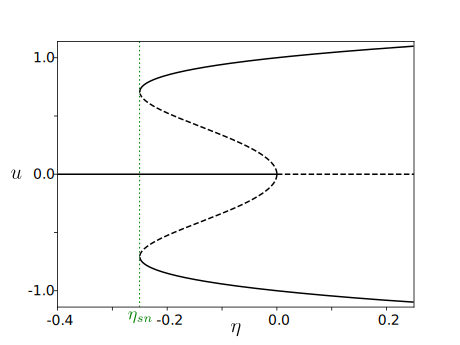
\includegraphics[width=0.6\textwidth]{imagenes/framework/bif_pitch_subcritical.pdf}
    \caption{Bifurcation diagram for the subcritical pitchfork. At the bifurcation point
    for $\eta=0$, two symmetric unstable branches emerge and gain stability after undergoing
    a saddle-node bifurcation for $\eta=\eta_{sn}$. The trivial solution is stable for $\eta < 0$
    and unstable for $\eta > 0$.}
    \label{fig:pre_bif_subpitchfork}
\end{figure}


\subsection{Andronov-Hopf bifurcation}

The two bifurcations discussed previously describe the emergence of steady states or fixed points. 
More specifically, they belong to the class of {\em stationary} bifurcations. Here, a different class of bifurcations will be introduced,
that of {\em dynamical} bifurcations, in which dynamical equilibria emerge. The simplest example is the Andronov-Hopf bifurcation
that allows for the emergence of a limit cycle or, in other words, a periodic equilibrium. Since oscillations are impossible in 
one dimension [ref strogatz], this bifurcation can only be present in systems of two or more dimensions. For simplicity, the following
analysis will be restricted to only two dimensions. However, it can easily be extended to the more general case of arbitrary dimensions.

\section{Localized Structures}
\label{sec:fra_LS}

\subsection{Solitons}

Among localized states, a particularly interesting type are solitons. They were discovered
 for the first time in 1834 by John Scott Russell. He described them 
 as a {\em "large solitary [...] heap of water, which continued its course along the channel without change of form
or diminution of speed"}[cita]. These solitary waves were highly controversial
at the time until Korteweg and de Vries provided an integrable model for shallow water waves
and proved their existence in the model [cita].
It was only a century later that the term soliton was coined by Zabusky and Kruskal
to emphasize their particle-like behavior after observing that solitons could pass through each
other with no change in shape or speed [cita]. Afterwards, the solitons were extensively studied
in other integrable and conservative equations such as the nonlinear Schrödinger
equation. In these systems, they arise due to a balance between dispersion and nonlinearity. 
More recently, the term dissipative soliton was coined to describe a similar localized state
in dissipative systems, where there is a continuous energy influx and dissipation. 
In these systems, they arise due to a balance between dispersion and nonlinearity. 


More recently, the term dissipative soliton was coined to describe a similar state
in dissipative systems, where there is a continuous energy influx and dissipation. 
In this context, an additional balance between gains and losses is required for the formation
of solitons. In what follows and, for the sake of simplicity, we shall use the term soliton
to refer to dissipative solitons as opposed to the original sense discussed previously
that is pertinent to conservative and integrable systems.



[dissipative soliton]

\subsection{Swift-Hohenberg equation}

\subsection{Resonant cavities and the Lugiato-Lefever equation}

\subsection{Non-local effects in the LLE}
\subsubsection{Raman effect}
\subsubsection{Spectral filtering}

\subsection{Spontaneous symmetry breaking and motion instabilities}

[normal, anomalous regime, MI etc]
[HOD, Raman]

\section{Phase oscillators and Chimera states}
\subsection{Phase oscillators}
\label{sec:phase_oscillators}

\subsection{Kuramoto model}

\subsection{Chimera states}

\subsection{Ott-Antonsen manifold reduction}